% Packaging
\section{Packaging}
\subsection{Test your application}
\begin{frame}[fragile]{Test your application}
    \begin{block}{Development}
        Run tests while developing using nose.
        \begin{minted}{bash}
python build.py test
        \end{minted}
    \end{block}
    \pause
    \begin{block}{Multi-environment}
        Once development is done, run tests against all different interpreters supported to check compatibility.
        \begin{minted}{bash}
python build.py tox
        \end{minted}
    \end{block}
    \pause
    \begin{block}{Continuous Integration}
        Development is done, tests pass in every environment, so code can be uploaded to repository safely. Once a commit is done:
        \begin{description}
            \item[Travis] run tests in every environment and will notify in case any test didn't pass. When all tests pass,
            \item[Coveralls] records current code coverage. In the same commit,
            \item[ReadTheDocs] gets the code, build docs and updates the project's doc page.
        \end{description}
    \end{block}
\end{frame}

\subsection{Creating a package}
\begin{frame}[fragile]{Package types}
    \begin{block}{Egg}
        Source distribution.
        \begin{minted}{bash}
python setup.py sdist
        \end{minted}
    \end{block}
    \pause
    \begin{block}{Wheel}
        Built and binary distribution.
        \begin{minted}{bash}
python setup.py bdist_wheel
        \end{minted}
    \end{block}
    \note{
        There is two types of python packages: \emph{egg} and \emph{wheel}. Source distribution needs a build step, built or binary distributions only need to move the package in the right path. Case of \emph{numpy}, \emph{scipy} and \emph{pandas}.
    }
\end{frame}

\begin{frame}{Builder}
    \begin{figure}
        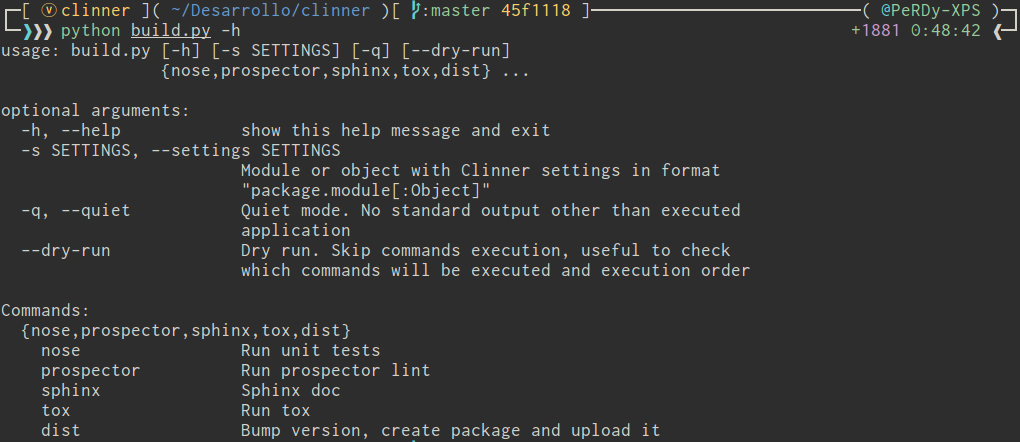
\includegraphics[width=\textwidth,height=0.8\textheight,keepaspectratio]{build_help.png}
    \end{figure}
\end{frame}

